% fig13_qstar_precision.tex — q* constant-fold precision: literal 2 pi/(mu0 R Ip)
% form |Delta|~5.8e-6 vs the pi-free q*=5 a^2 B/(R Ip) form |Delta|=0 (floored at
% machine epsilon ~1e-16 for the log axis). The constant-fold precision win.
% Compiled by the paper Makefile via `make figures` (pdflatex on the snippet).
%
% Data provenance (NO fabrication; commons @D g3) — Appendix F (app:bluemax:qstar):
%   literal form  q* = 2 pi a^2 B /(mu0 R Ip): the constant folder cannot fold the
%     transcendental pi, so 2 pi/(4 pi x 1e-7) cancels in floating point and leaves
%     a residue |Delta| ~ 5.8e-6 (middle-magnitude precision loss; NOT the float
%     floor ~1e-16, NOT a gross error -- enough to fail a tight formal epsilon).
%   pi-free form  q* = 5 a^2 B /(R Ip^MA): the integer 5 = 2 pi/(mu0 x 1e6) is
%     attested by q_star_constant (BLUE-MAX, |Delta|=0 exact). No transcendental
%     survives constant folding -> recompute |Delta|=0 on every input. Floored to
%     the IEEE-754 double epsilon ~1.1e-16 so the bar is visible on a log axis.
%
% Manual single-shot compile (debug):
%   pdflatex -interaction=nonstopmode -halt-on-error fig13_qstar_precision.tex
\documentclass[border=4pt]{standalone}
\usepackage{tikz}
\usepackage{pgfplots}
\pgfplotsset{compat=1.18}
\begin{document}
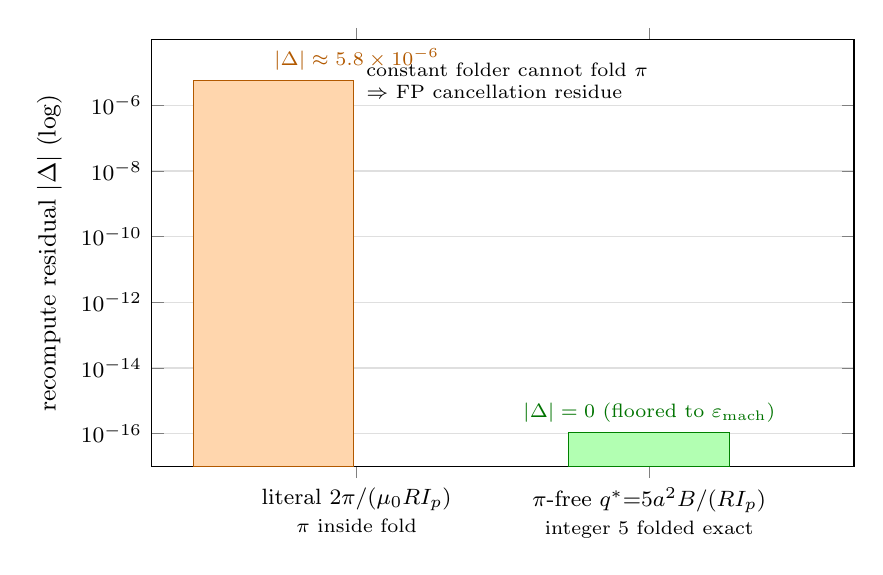
\begin{tikzpicture}
\begin{axis}[
  width=10.5cm, height=7cm,
  ybar,
  bar width=58pt,
  ymode=log,
  log origin=infty,
  ymin=1e-17, ymax=1e-4,
  ytick={1e-16,1e-14,1e-12,1e-10,1e-8,1e-6},
  ylabel={recompute residual $|\Delta|$ (log)},
  symbolic x coords={literal, pifree},
  xtick={literal, pifree},
  xticklabels={%
    \shortstack{literal $2\pi/(\mu_0 R I_p)$\\\scriptsize $\pi$ inside fold},
    \shortstack{$\pi$-free $q^*{=}5a^2B/(RI_p)$\\\scriptsize integer 5 folded exact}},
  x tick label style={font=\footnotesize,align=center},
  tick label style={font=\footnotesize},
  label style={font=\small},
  ymajorgrids,
  grid style={gray!25},
  enlarge x limits=0.7,
  clip=false,
]
% literal form: |Delta| ~ 5.8e-6 (transcendental does not fold)
\addplot[draw=orange!70!black,fill=orange!32] coordinates {(literal,5.8e-6)};
% pi-free form: |Delta| = 0, floored to IEEE-754 double epsilon ~1.1e-16 for log
\addplot[draw=green!50!black,fill=green!30,bar shift=0pt] coordinates {(pifree,1.1e-16)};
% annotations
\node[font=\scriptsize,text=orange!70!black,anchor=south] at (axis cs:literal,5.8e-6)
  {$|\Delta|\approx5.8\times10^{-6}$};
\node[font=\scriptsize,text=green!45!black,anchor=south] at (axis cs:pifree,1.1e-16)
  {$|\Delta|=0$ (floored to $\varepsilon_{\mathrm{mach}}$)};
\node[font=\scriptsize,text=black,anchor=north west,align=left]
  at (axis cs:literal,4e-5)
  {constant folder cannot fold $\pi$\\$\Rightarrow$ FP cancellation residue};
\end{axis}
\end{tikzpicture}
\end{document}
